%%
%% This is file `sample-sigconf.tex',
%% generated with the docstrip utility.
%%
%% The original source files were:
%%
%% samples.dtx  (with options: `sigconf')
%% 
%% IMPORTANT NOTICE:
%% 
%% For the copyright see the source file.
%% 
%% Any modified versions of this file must be renamed
%% with new filenames distinct from sample-sigconf.tex.
%% 
%% For distribution of the original source see the terms
%% for copying and modification in the file samples.dtx.
%% 
%% This generated file may be distributed as long as the
%% original source files, as listed above, are part of the
%% same distribution. (The sources need not necessarily be
%% in the same archive or directory.)
%%
%%
%% Commands for TeXCount
%TC:macro \cite [option:text,text]
%TC:macro \citep [option:text,text]
%TC:macro \citet [option:text,text]
%TC:envir table 0 1
%TC:envir table* 0 1
%TC:envir tabular [ignore] word
%TC:envir displaymath 0 word
%TC:envir math 0 word
%TC:envir comment 0 0
%%
%%
%% The first command in your LaTeX source must be the \documentclass
%% command.
%%
%% For submission and review of your manuscript please change the
%% command to \documentclass[manuscript, screen, review]{acmart}.
%%
%% When submitting camera ready or to TAPS, please change the command
%% to \documentclass[sigconf]{acmart} or whichever template is required
%% for your publication.
%%
%%
\documentclass[sigconf, anonymous, screen, review]{acmart}
\usepackage{array}
\usepackage{listings}
\usepackage{tikz}
\usetikzlibrary{shapes.geometric, arrows}
\definecolor{folderbg}{RGB}{124,166,198}
\definecolor{folderborder}{RGB}{110,144,169}
\lstset{escapechar=@}%aboveskip}=20pt,belowskip=20pt}
%\linespread{0.97}

%%
%% \BibTeX command to typeset BibTeX logo in the docs
\AtBeginDocument{%
  \providecommand\BibTeX{{%
    Bib\TeX}}}

%% Rights management information.  This information is sent to you
%% when you complete the rights form.  These commands have SAMPLE
%% values in them; it is your responsibility as an author to replace
%% the commands and values with those provided to you when you
%% complete the rights form.
\setcopyright{acmcopyright}
\copyrightyear{2023}
\acmYear{2023}
\acmDOI{XXXXXXX.XXXXXXX}

%% These commands are for a PROCEEDINGS abstract or paper.
\acmConference[CODASPY '23]{The 13th Conference on Data and Application Security and Privacy}{April 24--26,
  2023}{Charlotte, NC}
%%
%%  Uncomment \acmBooktitle if the title of the proceedings is different
%%  from ``Proceedings of ...''!
%%
%%\acmBooktitle{Woodstock '18: ACM Symposium on Neural Gaze Detection,
%%  June 03--05, 2018, Woodstock, NY}
\acmPrice{15.00}
\acmISBN{978-1-4503-XXXX-X/18/06}


%%
%% Submission ID.
%% Use this when submitting an article to a sponsored event. You'll
%% receive a unique submission ID from the organizers
%% of the event, and this ID should be used as the parameter to this command.
%%\acmSubmissionID{123-A56-BU3}

%%
%% For managing citations, it is recommended to use bibliography
%% files in BibTeX format.
%%
%% You can then either use BibTeX with the ACM-Reference-Format style,
%% or BibLaTeX with the acmnumeric or acmauthoryear sytles, that include
%% support for advanced citation of software artefact from the
%% biblatex-software package, also separately available on CTAN.
%%
%% Look at the sample-*-biblatex.tex files for templates showcasing
%% the biblatex styles.
%%

%%
%% The majority of ACM publications use numbered citations and
%% references.  The command \citestyle{authoryear} switches to the
%% "author year" style.
%%
%% If you are preparing content for an event
%% sponsored by ACM SIGGRAPH, you must use the "author year" style of
%% citations and references.
%% Uncommenting
%% the next command will enable that style.
%%\citestyle{acmauthoryear}


%%
%% end of the preamble, start of the body of the document source.
\begin{document}

%%
%% The "title" command has an optional parameter,
%% allowing the author to define a "short title" to be used in page headers.
\title{Guidelines to Improve the Delivery of Network Intrusion Detection Datasets}
\subtitle{Data/Toolset Paper}

%%
%% The "author" command and its associated commands are used to define
%% the authors and their affiliations.
%% Of note is the shared affiliation of the first two authors, and the
%% "authornote" and "authornotemark" commands
%% used to denote shared contribution to the research.
\author{Brian Lewandowski}
\email{balewandowski@wpi.edu}
\affiliation{%
  \institution{Worcester Polytechnic Institute}
  \streetaddress{100 Institute Road}
  \city{Worcester}
  \state{Massachusetts}
  \country{USA}
  \postcode{01609}
}

%\author{Randy Paffenroth}
%\email{rcpaffenroth@wpi.edu}
%\affiliation{%
%  \institution{Worcester Polytechnic Institute}
%  \streetaddress{100 Institute Road}
%  \city{Worcester}
%  \state{Massachusetts}
%  \country{USA}
%  \postcode{01609}
%}

%%
%% By default, the full list of authors will be used in the page
%% headers. Often, this list is too long, and will overlap
%% other information printed in the page headers. This command allows
%% the author to define a more concise list
%% of authors' names for this purpose.
\renewcommand{\shortauthors}{Lewandowski et al.}

%%
%% The abstract is a short summary of the work to be presented in the
%% article.
\begin{abstract}
    Applying deep learning techniques to perform network intrusion detection has expanded significantly in recent years.
    One of the main factors contributing to this expansion is the availability of improved network intrusion detection datasets.
    Despite recent improvements to these datasets, researchers have found it difficult to effectively compare methodologies across a wide variety of datasets due to the unique features generated as part of the delivered datasets.
    In addition, it is often difficult to generate new features using a dataset due to the lack of packet capture files or inadequate ground truth labeling information for a given dataset.
    In this work, we look at network intrusion dataset development with a focus on improving the delivery of datasets from a dataset researcher to a researcher acquiring the dataset for the research of anomaly detection and classification techniques.
    Specifically, we focus on making existing features more understandable, providing clear labeling criteria, and allowing a clear path for researchers to generate new features.
    We outline a set of guidelines for achieving these improvements along with providing a publicly available sample implementation that meets the guidelines using an existing network intrusion detection dataset.
\end{abstract}

%%
%% The code below is generated by the tool at http://dl.acm.org/ccs.cfm.
%% Please copy and paste the code instead of the example below.
%%
\begin{CCSXML}
<ccs2012>
<concept>
<concept_id>10002978.10003014</concept_id>
<concept_desc>Security and privacy~Network security</concept_desc>
<concept_significance>500</concept_significance>
</concept>
<concept>
<concept_id>10002978.10003022.10003023</concept_id>
<concept_desc>Security and privacy~Software security engineering</concept_desc>
<concept_significance>500</concept_significance>
</concept>
</ccs2012>
\end{CCSXML}

\ccsdesc[500]{Security and privacy~Network security}
\ccsdesc[500]{Security and privacy~Software security engineering}

%%
%% Keywords. The author(s) should pick words that accurately describe
%% the work being presented. Separate the keywords with commas.
\keywords{network intrusion detection, datasets, machine learning, deep learning}
%% A "teaser" image appears between the author and affiliation
%% information and the body of the document, and typically spans the
%% page.
%\begin{teaserfigure}
%  \includegraphics[width=\textwidth]{sampleteaser}
%  \caption{Seattle Mariners at Spring Training, 2010.}
%  \Description{Enjoying the baseball game from the third-base
%  seats. Ichiro Suzuki preparing to bat.}
%  \label{fig:teaser}
%\end{teaserfigure}

\received{17 October 2022}
%\received[revised]{12 March 2009}
%\received[accepted]{5 June 2009}

%%
%% This command processes the author and affiliation and title
%% information and builds the first part of the formatted document.
\maketitle

\section{Introduction}
Network intrusion detection (NID) is a methodology to protect computer networks by analyzing network traffic in order to identify malicious network traffic \cite{Chou2022}.
%In general, there exist two main strategies to perform network intrusion detection:  signature/behavior-based or anomaly-based \cite{yang2022systematic}.
%With signature-based detection, the network intrusion detection system (NIDS) attempts to identify malicious network traffic based on known attack patterns.
%Anomaly-based NIDS, however, excel at identifying malicious network behavior by detecting when network traffic strays beyond a baseline level of benign activity.
%This makes it more useful for the detection of zero-day attacks.
Researchers have begun to leverage machine and deep learning techniques in order to effectively combat the increasingly complex and evolving attacks taking place on networks today \cite{yang2022systematic}.
In order to properly research and verify the applicability of these data intensive techniques to network intrusion detection systems (NIDS), one must utilize datasets consisting of network scenarios that involve both benign and malicious activity.
To support these efforts a growing number of datasets have been developed such as those surveyed in \cite{Chou2022}, \cite{ring2019survey}, and \cite{yang2022systematic}.
Despite the great strides made in NIDS dataset development, researchers have identified limitations which make it hard to benchmark methods and expand on dataset features.
Some of these limitations include difficulty reproducing a dataset \cite{Chou2022}, \cite{ferriyan2021}; lack of a standard feature set \cite{sarhan_arxiv2021}, \cite{Sarhan2021}; and the inability to assess how a methodology generalizes across a broad set of datasets and scenarios \cite{sarhan2020netflow}, \cite{Sarhan2021}, \cite{wolsing2021ipal}.

\begin{figure*}
\centering
    \scalebox{0.99}{%
    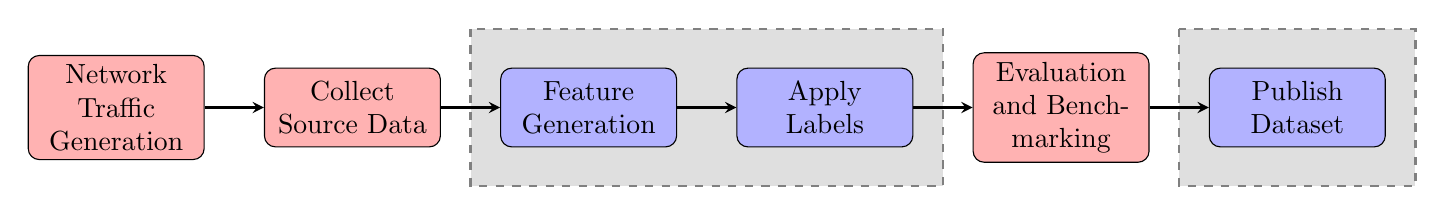
\begin{tikzpicture}
        \tikzstyle{process} = [rectangle, rounded corners, minimum width=2cm, minimum height=1cm,text centered, draw=black, fill=red!30, text width=2cm];
        \tikzstyle{processimp} = [rectangle, rounded corners, minimum width=2cm, minimum height=1cm,text centered, draw=black, fill=blue!30, text width=2cm];
        \tikzstyle{arrow} = [thick,->,>=stealth];
 
        \filldraw[fill=gray!25!white, draw=gray, thick, dashed] (4.5,1) rectangle (10.5,-1);
        \filldraw[fill=gray!25!white, draw=gray, thick, dashed] (13.5,1) rectangle (16.5,-1);
        \node(generate) [process] {Network Traffic Generation};
        \node(collect) [process, right of=generate, xshift=2cm] {Collect Source Data};
        \node(features) [processimp, right of=collect, xshift=2cm] {Feature Generation};
        \node(labels) [processimp, right of=features, xshift=2cm] {Apply Labels};
        \node(benchmark) [process, right of=labels, xshift=2cm] {Evaluation and Benchmarking};
        \node(publish) [processimp, right of=benchmark, xshift=2cm] {Publish Dataset};

        \draw[arrow] (generate) -- (collect);
        \draw[arrow] (collect) -- (features);
        \draw[arrow] (features) -- (labels);
        \draw[arrow] (labels) -- (benchmark);
        \draw[arrow] (benchmark) -- (publish);

    \end{tikzpicture}
    }

    \caption{
        An overview of the NID dataset development process.
        The areas that the guidelines seek to improve are depicted in blue with a gray background.
    }
    \label{fig:dataset_process}
\end{figure*}

In this work we propose both a set of guidelines along with a sample implementation of the guidelines to help dataset developers overcome these limitations.
The focus of the work presented here is to improve the handoff of a NIDS dataset to other researchers which has not been well explored in NIDS dataset research.
Figure \ref{fig:dataset_process} shows the dataset development process adapted from \cite{sarhan_arxiv2021} and \cite{e23111532} to show where this work logically fits. 
As can be seen highlighted in the figure, we focus on improvements for NIDS dataset feature and label generation which leads to additional improvements for the final delivery of the dataset.
More specifically, we provide a set of guidelines that can be used such that the end delivery of a NIDS dataset includes the original source network data as well as concrete scripts for generating each feature and label.
With both of these items in hand, researchers will be able to reliably recreate a dataset, ensure the same features are available across multiple datasets, and perform their own additional feature engineering.% using various NIDS datasets.

The main contributions of this work are as follows:

\begin{itemize}
    \item To the best of the authors' knowledge this is the first work to focus specifically on the handoff of NID datasets %from one researcher to another
    \item We identify examples seen in current research that hinder the handoff of NID datasets between researchers
    \item Guidelines are provided as a framework for overcoming limitations currently present in the NID dataset handoff process between researchers
    \item A sample implementation of the guidelines is presented along with publicly available source code\footnote{\linkanon{\url{https://github.com/WickedElm/nid\_dataset\_features\_framework}}}
\end{itemize}

The remainder of this work is outlined as follows.
In section \ref{sec:related_work} related works that look to improve the NIDS dataset development process are explored.
Section \ref{sec:characteristics} discusses the unique characteristics related to NID datasets that make the area challenging.
In section \ref{sec:nidddf} we discuss the details of our proposed guidelines including a sample implementation.
We conclude and outline future work in Section \ref{sec:conclusion}.

\section{Related Work}\label{sec:related_work}

The publicly available NID datasets that have been developed by researchers are well explored and analyzed in the literature through surveys such as \cite{Chou2022}, \cite{ring2019survey}, and \cite{yang2022systematic}.
These surveys break down the various datasets by different criteria such as data format, real versus synthetic data, availability, as well as statistical data regarding the datasets.
Other works seek to compare the value of various features delivered with NID datasets \cite{7809531}.
%In \cite{7809531}, the features of the KDD99 \cite{kdd99} and UNSW-NB15 \cite{unswnb15} datasets are compared and it is shown that the features provided with the UNSW-NB15 dataset provide a lower false alarm rate (FAR).
%Similarly, \cite{sarhan2020netflow} compares custom features from several datasets to using a standard set of features based on the NetFlow v9 protocol \cite{netflowv9format} in a work that makes datasets using the NetFlow v9 features available for public use.
Custom features from several datasets are compared to a standard set of features based on the NetFlow v9 protocol \cite{netflowv9format} in \cite{sarhan2020netflow}.

In a recent series of papers, Sarhan et al. explore limitations of current datasets and the impact these limitations have on evaluating methods across multiple networks and transitioning research into practical applications \cite{sarhan2020netflow}, \cite{sarhan2021cyber}, \cite{Sarhan2021}, \cite{sarhan_arxiv2021}.
The main limitation explored in these works include the fact that with such varied features included with delivered datasets, one cannot reliably compare a methodology across multiple networks to test for generalizability.
In addition, the works discuss how this hinders the transition from research to practical applications. 
%In response to these limitations, \cite{sarhan2020netflow} takes several benchmark datasets and transforms them into a common feature set based on NetFlow v9 consisting of 12 features.
%This set of features is expanded in \cite{Sarhan2021} to include 43 features based on the NetFlow v9 standard.
%Compared to the original set of features generated in \cite{sarhan2020netflow}, using the expanded feature set for classification generally produced superior results.
%In \cite{sarhan2021cyber}, this expanded feature set is used to perform federated learning across multiple datasets to simulate using data from several different networks to inform a centralized model.
%Finally, in \cite{sarhan_arxiv2021}, multiple common benchmark datasets are compared using the expanded NetFlow feature set and a set of features generated using CICFlowMeter \cite{lashkari2017characterization} in order to evaluate the relative performance of two standard feature sets generated from the same base network data.

Our work looks to build off of that published by Sarhan et al. in order to enable researchers to overcome these identified limitations.
%Rather than defining a standard feature set, we aim to make it easier for researchers to provide a dataset that is reproducible in terms of features and easily expanded or adjusted.
We aim to make it easier for researchers to provide a dataset that is reproducible from source data and easily expanded or adjusted.
In this way, one could easily use a standard feature set as well as research augmenting such a feature set for improvements.

The work in \cite{ferriyan2021} introduces the HIKARI-2021 dataset which focuses on including encrypted data as part of its dataset.
In addition, a set of content and process requirements are presented for generating a reproducible dataset.
The content requirements outlined includes providing full packet capture (PCAP) files, including full data payload, anonymizing real traffic,  providing ground truth data, using up-to-date traffic, labeling the data, and providing information regarding encryption.
The process requirements pertain to information that should be provided in order to make generating the dataset reproducible.
%While we agree with much of this work, we look to extend these concepts by requiring actual scripts to generate features and perform labeling along with full PCAP files.
We agree with these concepts and look to extend them by proposing the inclusion of actual scripts to generate features and perform labeling along with full PCAP files.
This leaves no ambiguity in descriptions for how to regenerate a dataset.
%As an example Zeek\footnote{https://zeek.org/} was used to extract the features for HIKARI-2021, however, no Zeek scripts were provided such that all features can be reproduced properly by researchers downstream.

While not the main focus, both \cite{e23111532} and \cite{layeghy2021} discuss and tackle the need to use a common feature set for comparison of their methods as opposed to using proprietary features delivered with most NID datasets available today.
Both provide informative descriptions regarding the features used in their work.
In addition, \cite{layeghy2021} provides the actual calculations for the features used in their work.
We believe this is a step in the right direction for the level of detail necessary to reproduce datasets from source data. 
%In this work, we advocate to naturally extend this information into scripts that are provided along with source network captures to make reproduction and extending the dataset more accessible and leave less room for error.
We seek to naturally extend this information into scripts that are provided along with source network captures to make reproduction and extending the dataset more accessible and leave less opportunity for error.

The survey presented in \cite{Chou2022} covers NID with a focus on datasets and their associated challenges.
A discussion on the reproducibility of methods found in research using public datasets is presented.
Here, it is shown that there are copious examples of research that is not reproducible either due to code not being available, portions of code that is missing, or code that is too unique to an individual researcher's environment.
The focus of these critiques were on research performed using NID datasets.
We believe using the guidelines outlined in our work will reduce these types of errors by enabling the development of datasets that have a clear path for being handed off from one researcher to another.

%%The work in \cite{9787094} presents Reliable-NIDS (R-NIDS) as a system for working with multiple integrated datasets.
%The work in \cite{9787094} presents a system for working with multiple integrated datasets.
%%The method is used to produce the UNK22 dataset, which is a combination of several well known existing datasets.
%%The premise of \cite{9787094} is that research assessed across a single NID dataset does not indicate that it will generalize across different networks reliably.
%The premise of \cite{9787094} is that research assessed across a single NID dataset does not indicate that it will generalize across different networks reliably.
%The authors point to the fact that NID datasets have both different feature sets and formats for the data.
%%As a solution to this, the work presents a complete system that uses a method called Feature as a Counter to combine multiple NID datasets into a single dataset.
%We agree with the premise of this work and believe that our work will be an additional step towards minimizing the difficulties in combining multiple datsets together.

%\section{Unique Characteristics of Network Intrusion Detection Datasets}\label{sec:characteristics}
\section{Characteristics of NID Datasets}\label{sec:characteristics}
%There are several characteristics unique to generating NID datasets that make the downstream hand off of them difficult compared to other dataset types.
In this section we briefly discuss the characteristics unique to generating NID datasets that make the downstream hand off of them difficult compared to other dataset types.
%Here we briefly discuss several of those characteristics.

%\subsection{Infrastructure Constraints Affect Data Collection}\label{subsec:infrastructure}
\subsection{Infrastructure Constraints}\label{subsec:infrastructure}
Researchers generally consider collecting real data, simulated data, or a mix of the two when generating a NID dataset \cite{Chou2022}, \cite{ring2019survey}. 
In each of these scenarios, there are constraints imposed on the data collection that affect the amount of data collected as well as the format used for collection.

When collecting real network data from an existing network we are generally limited by the current network structure that is in place.
This includes the network architecture, the size of the network, and the equipment being used.
Depending on the amount of network traffic as well as storage devices available, it may not be feasible to collect all network data in PCAP format.
This results in some information being lost at the collection point when using alternatives such as NetFlow.
When considering flow data, we may be limited to a specific version of NetFlow, such as v5, or having only a subset of attributes available for collection.
In addition, it is unlikely that researchers can execute attacks on a true live network.
This leaves such collections having an unknown mix of benign and potentially malicious network activity requiring in-depth analysis for labeling.
In many live network situations, some data may need to be redacted or anonymized for privacy purposes.

To have more control over the collection environment, researchers often choose to generate simulated network traffic using traffic generation tools in combination with a dedicated network lab \cite{unswnb15}, \cite{sharafaldin2018toward}.
In these cases, more control is had over the network architecture being simulated and issues such as introducing attacks and labeling data are overcome more easily than a live scenario.
Even in this scenario, however, one needs to be mindful of how much storage and compute power the facility has available for the task.
In addition, researchers must take care to assess the quality of the simulated scenario in terms of how well it emulates the same attack in a real world setting.

When combining both simulated and live data together for a NID dataset, researchers have a blend of high quality live network data in combination with a controlled attack scenario.
Despite these benefits, one must still consider the constraints for both settings.

%\subsection{Collected Data Formats Not Suitable for Machine Learning}\label{subsec:collectionformat}
\subsection{Data Formats Not Suitable for Model Input}\label{subsec:collectionformat}
Unlike many other areas of research, the collected data format for network data is not in a format suitable for ingestion by a deep learning model for training.
The PCAP and NetFlow collection format is binary in nature and does not translate well for machine learning.
In addition, included in the data are both categorical and numerical features making the problem harder than when compared to other binary formats such as image data. 
For example, with image data, one can directly translate all of the data to numerical values for ingestion by a model.
For PCAP and NetFlow files, direct translations from an IP address to a numerical value risks losing information regarding similarities between hosts \cite{ringip2vec}.
In response to this, dataset researchers generally process the binary source data after collection in order to generate a set of ingestible features.

This generally introduces multiple decision points for a dataset researcher to consider such as delivering all packet data in an ingestible format or summarizing the data into flow data. 
In both cases, one must consider which features to provide and in the case of flow data, which version (if any) is used.
All of the decisions made at this point are generally valid and at the discretion of the researcher but they introduce the potential to inhibit further progress for other researchers intrested in using the dataset.
As discussed later in Section \ref{sec:intrinsic_value}, this is often where the activities of producing a NID dataset and performing feature engineering are combined into the same activity when it may be more beneficial to explicitly separate them.

\subsection{Varied Standard Data Formats}\label{subsec:nostandard}
When considering the collection of network data there are several standard formats to consider.
These include PCAPs, various versions of NetFlow, and IPFIX \cite{claise2008specification}.
In addition to these standard formats, there may also be network hardware that only support vendor standards.
While always collecting full packet captures is ideal in terms of retaining all information, it is often unfeasible due to the volume of data being produced.

When turning to a flow format, challenges are imposed on NID dataset developers as some facilities may be using the NetFlow v5 standard while others may have upgraded to NetFlow v9 or IPFIX.
Any limitations or differences between the standards will trickle down into the final delivered datasets resulting in datasets with varied features such that researchers cannot rely on a particular feature always being present in a dataset for their work.
%While the recent introduction of the Open Cybersecurity Schema Framework (OCSF)\footnote{https://github.com/ocsf/} looks to improve this situation, it is unclear when wide support will be available for this  standard to be used in practice.

\section{NID Dataset Delivery Guidelines}\label{sec:nidddf}

%\section{Recognizing the Intrinsic Value in Network Intrusion Detection Datasets}\label{sec:intrinsic_value}
\subsection{The Intrinsic Value in NID Datasets}\label{sec:intrinsic_value}
We believe it is worthwhile to provide a brief discussion regarding the intrinsic value provided by NID datasets as related to their development and subsequent distribution.
Namely, the intrinsic value of a NID dataset is created during the scenario development, execution, and \textit{source data} collection and not by the final delivered features.
To be clear, the final features are valuable, but they are representative of a separate feature engineering activity that takes place after the intrinsic value of a network scenario has been captured in source data.
In other words, the value provided by the NID dataset is derived from the actual network intrusion scenario and its collected source data. 
A researcher could provide any number of derived features with varying degrees of value for attack detection, however, the intrinsic value of the source data remains constant as it is derived from the scenario that was captured.

One goal of this framework is to highlight these two separate activities by advocating for the delivery of both source data and separate scripts that generate the features that take place during any subsequent feature engineering.
Providing both items delivers the value of both activities to downstream researchers.


\subsection{Guidelines Details}\label{subsec:framework_overview}
The main ideas behind the proposed guidelines are simple in statement but oftentimes overlooked in practice.
Specifically considering the hand off of datasets from one researcher to another; the guidelines focus on ease of access, reproducibility from source data, verification, and extension.
The guidelines are meant to provide general guidance for making the delivery of NID datasets meet these four areas of focus.
We note that implementations of the guidelines will differ due to the variety of tools that researchers use to generate their datasets.
As discussed further in Section \ref{sec:conclusion}, we aim to provide a remedy for implementation differences in future work.
In addition, it is important to make the distinction that when we reference reproducibility of a dataset, we refer to reproducing the dataset's final features from the original source data as opposed to recreating and re-executing the dataset's NID scenario.

The ten guidelines are outlined and described in Table \ref{tbl:guidelines}.
Guidelines one through four pertain to providing downstream researchers with the resources necessary to actively reproduce and enhance the provided dataset.
Guidelines five through nine outline steps that can be taken to ensure that all of the dataset features and labels can be regenerated from source data and that the steps for this generation of features can be verified and understood by downstream researchers.
Finally, guideline ten is specifically included to emphasize that the delivered datasets can be considered active projects and adjust over time for any errors found after initial presentation to researchers.
Collectively, these guidelines are proposed to help avoid situations such as with the KDD Cup '99 \cite{kdd99} and CICIDS2017 datasets \cite{sharafaldin2018toward}, where researchers have found issues with the original datasets resulting in multiple variants of the dataset being available with specific corrections \cite{tavallaee2009detailed}, \cite{lanvin:hal-03775466}, \cite{engelen2021}.

\begingroup
\setlength{\tabcolsep}{10pt} % Default value: 6pt
\renewcommand{\arraystretch}{2.0} % Default value: 1
\begin{table*}
\centering
\caption{
    Guidelines for improving the delivery of NID datasets from dataset researchers to downstream researchers.
}
\label{tbl:guidelines}
%\resizebox{\columnwidth}{!}{%
%\begin{tabular}{|l|c|c|c|c|c|}
\begin{tabular}{m{8cm} m{8cm}}
    \hline
    \textbf{Guideline} & \textbf{Details} \\
    \hline

    \textbf{(1) Provide direct access to all data and scripts for dataset} & 
    \begin{itemize}
        \item Provide a download script
        \item Avoid barriers to download such as requiring logins or filling out forms
    \end{itemize} \\

    \textbf{(2) Include complete source data to the most detailed extent possible} &
    \begin{itemize}
            \item Full PCAP
            \item Partial PCAP
            \item Full Network Flow data
            \item Partial Network Flow data
        \end{itemize} \\

    \textbf{(3) If possible, provide access to all tools needed to generate dataset} &
    \begin{itemize}
        \item Provide a container environment or virtual machine
    \end{itemize} \\

    \textbf{(4) Provide documentation indicating how to reproduce a dataset from source data} &
        \begin{itemize}
            \item Provide commands needed to execute scripts
            \item Identify specific versions of tools required
        \end{itemize} \\

    \textbf{(5) Include source code needed to reproduce dataset features} &
    \begin{itemize}
        \item Avoid making code too specific to a given user environment
        \item Following guideline (3) may help to avoid environment differences
    \end{itemize} \\

    \textbf{(6) The source code for each feature should be easily identifiable} &
    \begin{itemize}
        \item Consider naming conventions that match the final  feature name
        \item Consider a separate script, code unit, or identifier for each feature
    \end{itemize} \\

    \textbf{(7) The generation of each feature should be independent from others} &
    \begin{itemize}
        \item Makes the specific code that creates each feature more understandable and reviewable
        \item Avoids execution dependencies between features
        \item Facilitates the ability to remove or add new features by downstream researchers
    \end{itemize} \\

    \textbf{(8) Apply guidelines outlined for features to labels as well} &
    \begin{itemize}
        \item Treat labels the same as other features by applying guidelines (4), (5), and (6) for any labels applied to the data
        \item While labels are significant for model training, during dataset generation time, they are simply a special case of features
    \end{itemize} \\

    \textbf{(9) Make source code for labeling distinct from other features} &
    \begin{itemize}
        \item Having source code for labeling provides important insight for downstream researchers making it important to easily identify
        \item The labeling procedure and/or criteria can indicate features to avoid using in models.
              For example, if the labeling criteria is based on a single IP address, it is likely that IP address should not be provided to a model.
    \end{itemize} \\

    \textbf{(10) Provide a mechanism to receive and implement feedback from researchers to correct issues and improve dataset} &
        \begin{itemize}
            \item Allows dataset to remain current
            \item Prevents multiple variations of the same dataset from being developed by different researchers for corrected issues
            \item Consider using version control on the source code used to generate the dataset
        \end{itemize} \\
    \hline
\end{tabular}
%}
\end{table*}
\endgroup

\subsection{Sample Implementation}\label{subsec:framework_implementation}
The main details of the environment used to develop and test this sample implementation can be found in the $documentation$ section of the provided $./config/unsw\text{-}nb15.yaml$ file.
It is assumed that any usage of it would be in a similar environment.

%\begingroup
%\setlength{\tabcolsep}{10pt} % Default value: 6pt
%\renewcommand{\arraystretch}{1.5} % Default value: 1
%\begin{table}
%\centering
%\caption{
%Table of the software environment that the sample implementation was developed and tested on.
%To replicate its execution one would need to have a similar environment.
%}
%\label{tbl:software_environment}
%%\resizebox{\columnwidth}{!}{%
%%\begin{tabular}{|l|l|l|l|}
%\begin{tabular}{ll}
%    \hline
%    \textbf{Software} &  \textbf{Version} \\
%    \hline
%    Ubuntu & 18.04 \\
%    Bash & 4.4.20 \\
%    Python & 3.8.10 \\
%    Zeek & 4.2.1 \\
%    Argus & 3.0.8.2 \\
%    \hline
%\end{tabular}
%%}
%\end{table}
%\endgroup

\subsubsection{Overview}\label{subsubsec:sample_overview}
We provide a sample implementation of the guidelines outlined in Section \ref{subsec:framework_overview} which can be used and adapted by NID dataset researchers.
While this specific implementation makes use of Zeek\footnote{\url{https://zeek.org/}} and Argus\footnote{\url{https://openargus.org/}} in combination with Python\footnote{\url{https://www.python.org/}}, we note that any toolchain which sufficiently implements the guidelines would achieve the same goals of providing ease of access, reproducibility from source data, verification, and extension.
We used a small portion of the UNSW-NB15 dataset \cite{unswnb15} as the source data for this implementation as this dataset provides open access to all of its source data.
Note that some choices for this implementation were made to specifically exercise usage of the guidelines and that the resulting dataset is for example purposes.
Therefore, our example dataset should not be used for researching NID techniques.

We based our sample implementation of the guidelines on characterizing the creation of a deliverable dataset from source data into four main areas:  acquiring source data, feature processing, label processing, and final dataset processing.
Using YAML\footnote{\url{https://yaml.org/}} for the format of our input files for the implementation we see these main areas depicted in Listing \ref{lst:yamltemplate}.
In the documentation section of this file, one can indicate all of the versions of tools used.
The setup\_options section is in place for dealing with construction complexities such as needing to resolve paths and indicating where to store artifacts.
The remaining sections handle our four main areas of concern and are intended to explicitly be populated with the commands that will be executed to generate a dataset from source files.
The $step\_acquire\_source\_data$ section would generally consist of commands or scripts to automate the downloading of source data from a remote site.
Both the $step\_feature\_processing$ and $step\_label\_processing$ sections contain sub-sections corresponding to what level of detail is being used for the given feature or label.
Features that require inspecting individual packets would be considered $packet\_level$, features that are derived from a single NetFlow entry would be considered $flow\_level$, and features requiring access to multiple flows or higher level data would be considered to be at the $network\_level$.
While the functions contained under the $step\_final\_dataset\_processing$ will likely vary widely for different situations, we expect this section would consist of merging various features created by different tools such that they can be delivered in a single file or set of files with a consistent format.
The YAML configuration file is read in by python code and commands are executed from the top down.

Excluding the $documentation$ and $setup\_options$ sections, the sample implementation is set up with a directory structure that mirrors the remaining sections of the input YAML file.
The contents of these directories correspond to scripting and configuration data for the respective step.
Doing this makes it easy for researchers to find the scripts they are interested in examining and updating.

\subsubsection{Basic Usage}\label{subsubsec:basic_usage}
After downloading the sample source code, one can change to its top level directory and execute the command in Listing \ref{lst:maincmd} to create the sample dataset.
This command calls our main script, $create\_dataset.py$; passing in the path to the YAML file to be processed.
The $create\_dataset.py$ script reads in the file, performs variable replacements, and then simply executes all of the commands contained  in the file.
After running the script, one will see a new directory, $unsw\_nb15\_dataset$, has been created.
This directory contains the final output file, $unsw\_nb15\_dataset.csv$, along with various intermediate state files.
All of these names can be updated by editing the input YAML configuration file.

\noindent\begin{minipage}{\linewidth}
\begin{lstlisting}[aboveskip=10pt, label=lst:yamltemplate, caption={A template input file for our sample guidelines implementation.  Each section would be filled in with either information or explicit commands that get run to generate a feature set from network source data.}, captionpos=b, basicstyle=\footnotesize, backgroundcolor=\color{gray!10!white}, frame=stb]
   documentation:
   
   setup_options:
   
   step_acquire_source_data:
   
   step_feature_processing:
     packet_level:
     flow_level:
     network_level:
   
   step_label_processing:
     packet_level:
     flow_level:
     network_level:
   
   step_final_dataset_processing:
\end{lstlisting}
\end{minipage}


\begin{lstlisting}[label=lst:maincmd, caption={The command to run to execute the sample implementation of the guidelines.}, captionpos=b, basicstyle=\footnotesize, backgroundcolor=\color{gray!10!white}, frame=stb, breaklines=True]
python ./src/create_dataset.py \
    ./config/unsw-nb15.yaml
\end{lstlisting}


\subsubsection{Supporting Multiple Tools}\label{subsubsec:tool_support}
There are many tools used for working with network data and so this sample implementation provides basic support for several of them to serve as an example of this common scenario.
In this example, we support tools using a combination of simple wrapper scripts for each tool and minimal tool specific infrastructure.
Each wrapper script reads in a simple configuration file which consists of a listing of feature/label specific procedures that are to be executed by the given tool.
These configuration files have a naming convention of $\_\_load\_\_.<tool>$.
A sample of these files can be seen in Figure \ref{fig:sample_load_files}.
For both Zeek and Python, the entries in these configuration files refer to a Zeek and python script respectively.
The entries in the configuration files for Argus correspond to a field passed to the Argus client as part of the field identifier option.
In addition, the Zeek scripting is supported by the implementation of a new Zeek package located in our source code the under $./src/zeek/packages$ directory.

\begin{figure}
\centering
    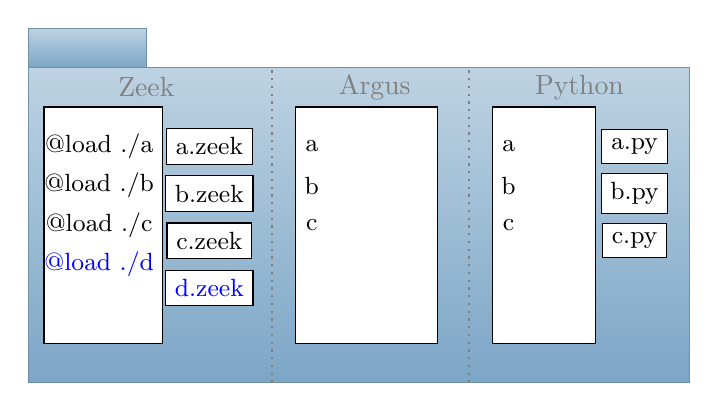
\begin{tikzpicture}
        \tikzstyle{directory} = [rectangle, draw=folderborder, top color=folderbg!50, bottom color=folderbg, minimum width=8.4cm, minimum height=4.0cm];
        \tikzstyle{directorytop} = [rectangle, draw=folderborder, top color=folderbg!50, bottom color=folderbg, minimum width=1.5cm, minimum height=0.5cm];

        \node(zeekdir) [directory] {};
        \node(zeekdirtop) [directorytop, above of=zeekdir, xshift=-3.45cm, yshift=1.25cm] {};
        \filldraw[fill=white, draw=black] (-4, -1.5) rectangle (-2.5,1.5);
        \node[] at (-3.3, 1) {\small @load ./a};
        \node[] at (-3.3, 0.5) {\small @load ./b};
        \node[] at (-3.3, 0) {\small @load ./c};
        \node[text=blue] at (-3.3, -0.5) {\small @load ./d};

        \node[fill=white, draw=black] at (-1.9, 1) {\small a.zeek};
        \node[fill=white, draw=black] at (-1.9, 0.4) {\small b.zeek};
        \node[fill=white, draw=black] at (-1.9, -0.2) {\small c.zeek};
        \node[fill=white, draw=black, text=blue] at (-1.9, -0.8) {\small d.zeek};

        \filldraw[fill=white, draw=black] (-0.8, -1.5) rectangle (1,1.5);
        \node[] at (-0.6, 1) {\small a};
        \node[] at (-0.6, 0.5) {\small b};
        \node[] at (-0.6, 0) {\small c};

        \filldraw[fill=white, draw=black] (1.7, -1.5) rectangle (3, 1.5);
        \node[] at (1.9, 1) {\small a};
        \node[] at (1.9, 0.5) {\small b};
        \node[] at (1.9, 0) {\small c};

        \node[fill=white, draw=black] at (3.5, 1) {\small a.py};
        \node[fill=white, draw=black] at (3.5, 0.4) {\small b.py};
        \node[fill=white, draw=black] at (3.5, -0.2) {\small c.py};

        \draw[draw=gray, thick, dotted] (-1.1,-2) -- (-1.1,2);
        \draw[draw=gray, thick, dotted] (1.4,-2) -- (1.4,2);

        \node[text=gray] at (-2.7, 1.75) {Zeek};
        \node[text=gray] at (0.2, 1.75) {Argus};
        \node[text=gray] at (2.8, 1.75) {Python};

    \end{tikzpicture}

    \caption{
        A typical directory for feature scripts that will be executed using our implementation's wrapper scripts.
        The large white boxes consist of the contents of the $\_\_load\_\_.<tool>$ configuration files.
        Alongside them are the corresponding scripts that would be found in the directory.
        The wrapper scripts read the $\_\_load\_\_.<tool>$ file and executes the corresponding scripts.
        For Argus there is only the configuration file as its entries correspond to command line arguments to be used as input to the Argus client tool.
        Depicted with blue text is a new feature made by a downstream researcher which will be generated using the Zeek tool.
    }
    \label{fig:sample_load_files}
\end{figure}

\subsubsection{Adding and Removing Features}\label{subsubsec:adding_removing_features}
%With the tool support infrastructure in place, this sample makes it straightforward to identify which features are to be created and augment those features easily.
With the tool support infrastructure in place, it is straightforward to augment the original feature set.
The creation of any new feature requires two main steps:  updating the appropriate $\_\_load\_\_.<tool>$ file and then creating the corresponding feature script if necessary for the particular tool being used.
For example, if one wanted to create a new flow level feature using Zeek, one would create their new Zeek script in the $./src/step\_feature\_processing/flow\_level$ directory and update that directory's $\_\_load\_\_.zeek$ file with the script's name as depicted in Figure \ref{fig:sample_load_files} in blue text.
For Zeek scripts, we have set up a template that can be followed for creating features using specific callbacks available within its scripting framework.
Removing a feature is a simple task of finding the appropriate $\_\_load\_\_.<tool>$ file and either removing the name of the feature from the listing in the file or commenting out the line using an octothorpe.
Note that these same procedures are applied for labeling procedures, however, they have separate configuration files.

%\begin{figure}
%\centering
%    \begin{tikzpicture}
%        %\tikzstyle{directory} = [rectangle, minimum width=2.5cm, minimum height=3cm,text centered, draw=black, fill=red!30, text width=2cm];
%        \tikzstyle{directory} = [rectangle, draw=folderborder, top color=folderbg!50, bottom color=folderbg, minimum width=4cm, minimum height=3.5cm];
%        \tikzstyle{directorytop} = [rectangle, draw=folderborder, top color=folderbg!50, bottom color=folderbg, minimum width=1cm, minimum height=0.5cm];
%        \tikzstyle{arrow} = [thick,->,>=stealth];
%
%        %\filldraw[draw=folderborder, top color=folderbg!50, bottom color=folderbg] (0,4) rectangle (1,3.5);
%        %\filldraw[draw=folderborder, top color=folderbg!50, bottom color=folderbg] (0,0) rectangle (3,3.5);
%
%        \node(beforedir) [directory] {};
%        \node(beforedirtop) [directorytop, above of=beforedir, xshift=-1.5cm, yshift=1.0cm] {};
%        \filldraw[fill=white, draw=black] (-1.9, -1.5) rectangle (0.0,1.5);
%        \node[] at (-1, 1) {@load ./a};
%        \node[] at (-1, 0.5) {@load ./b};
%        \node[] at (-1, 0) {@load ./c};
%
%        \node[fill=white, draw=black] at (0.75, 1) {a.zeek};
%        \node[fill=white, draw=black] at (0.75, 0.4) {b.zeek};
%        \node[fill=white, draw=black] at (0.75, -0.2) {c.zeek};
%
%        \node(afterdir) [directory, right of=beforedir, xshift=4cm] {};
%        \node(afterdirtop) [directorytop, above of=afterdir, xshift=-1.5cm, yshift=1.0cm] {};
%        \filldraw[fill=white, draw=black] (3.1, -1.5) rectangle (5,1.5);
%        \node[] at (4.0, 1) {@load ./a};
%        \node[] at (4.0, 0.5) {@load ./b};
%        \node[] at (4.0, 0) {@load ./c};
%        \node[text=blue] at (4.0, -0.5) {@load ./d};
%
%        \node[fill=white, draw=black] at (5.75, 1) {a.zeek};
%        \node[fill=white, draw=black] at (5.75, 0.4) {b.zeek};
%        \node[fill=white, draw=black] at (5.75, -0.2) {c.zeek};
%        \node[fill=white, draw=black, text=blue] at (5.75, -0.8) {d.zeek};
%
%        \draw [->,blue,thick,>=stealth] (beforedirtop.north) to [out=30,in=150] (afterdirtop.north);
%
%    \end{tikzpicture}
%
%    \caption{
%        Example of adding a new feature using our sample implementation of the guidelines.
%        The original directory on the left is augmented in two ways with changes shown in blue text.
%        First, a new Zeek script based on our template is added to the directory called $d.zeek$.
%        Next, the $\_\_load\_\_.zeek$ file is augmented to include the new feature.
%    }
%    \label{fig:new_feature_process}
%\end{figure}

\section{Conclusion and Future Work}\label{sec:conclusion}
In this work we propose a set of ten guidelines that will improve the handoff of NID datasets between researchers.
The focus of these guidelines is to improve ease of access, reproducibility from source data, verification, and the extension of datasets.
We believe that considering these areas while generating new datasets will benefit both dataset developers and researchers using these datasets for further research.
%In addition, we provided an example implementation that follows these guidelines to demonstrate its benefits.
An example implementation was provided to demonstrate the benefits of these guidelines.

While these guidelines are a step forward in progress in this area of research, it does not eliminate many of the complexities faced by researchers who want to extend datasets.
In future work we aim to remove many of these complexities by using server based methods to facilitate these guidelines.
This future work would eliminate the burden of researchers having to acquire specific versions of tools and provide efficiency gains for distributing new features.

%% Acknowledgements for Professor Paffenroth
\begin{acks}
    We would like to acknowledge Professor Randy Paffenroth for his insights and guidance which helped shape this work.
\end{acks}

%%
%% The next two lines define the bibliography style to be used, and
%% the bibliography file.
\bibliographystyle{ACM-Reference-Format}
\bibliography{citations.bib}

\appendix
\section{Extended Code Listings}

\begin{minipage}{\linewidth}
\subsection{Sample Zeek Script}
\begin{lstlisting}[label=lst:zeeksamplescript, caption={
    A sample Zeek script that creates the single feature for source bytes.
    This script would be identified in a $\_\_load\_\_.zeek$ file and executed using the Zeek wrapper script provided by our sample implementation.
    Each script provides the feature name and implements supported Zeek callback functions.
    While we provide a default set of callbacks, others could  be added to this file if needed.
    One can see that breaking up the features into their own code unit makes understanding how they are generated straightforward.
    }, captionpos=b, basicstyle=\small, backgroundcolor=\color{gray!10!white}, frame=stb, breaklines=True]

   module Sbytes;
   
   ###
   # Add new feature to the connection record
   ###
   
   export {
       redef record Features::Info += {
           sbytes: count &log &optional;
       };
   }
   
   ###
   # Specify any namespace variables
   ###
   
   ###
   # Event handlers for feature
   ###
   
   event new_connection(c: connection) {
   
   }
   
   event new_packet(c: connection, p: pkt_hdr) {
   
   }
   
   event connection_state_remove(c: connection) &priority=-10
   {
       Features::connection_data[c$uid]$sbytes = c$conn$orig_bytes;
   }
\end{lstlisting}
\end{minipage}


\subsection{Fully Populated Sample YAML File}
Listing \ref{lst:populatedyaml} shows the fully populated YAML file developed for this sample implementation of the guidelines.

\begin{lstlisting}[float=*, label=lst:populatedyaml, caption={
    The fully populated YAML file used as input for our sample implementation.
    Making the scripting calls available for inspection leaves no ambiguity regarding how a final dataset is generated from the original source data.
    }, captionpos=b, basicstyle=\tiny, backgroundcolor=\color{gray!10!white}, frame=stb, breaklines=True]

   documentation:
     operating_system: Ubuntu 18.04
     python_version: 3.8.10
     zeek_version: 4.2.1
     argus_version: 3.0.8.2
     ra_client_version: 3.0.8 
     expected_outputs: 
       - unsw_nb15_dataset.csv
   
   setup_options:
     current_directory: ENV_PWD
     working_directory: ENV_PWD/unsw_nb15_dataset
   
   step_acquire_source_data:
     - python src/step_acquire_source_data/downloader.py ${setup_options.working_directory}
   
   step_feature_processing:
     packet_level:
       - rm -f ${setup_options.working_directory}/17-2-2015_1.argus
       - argus -S 60 -m -r ${setup_options.working_directory}/17-2-2015_1.pcap -w ${setup_options.working_directory}/17-2-2015_1.argus
       - ./src/argus/ra_wrapper.bash ${setup_options.working_directory} 17-2-2015_1.argus argus_features.csv ./src/step_feature_processing/packet_level/__load__.argus
   
     flow_level:
       - ./src/zeek/zeek-wrapper.bash ${setup_options.current_directory}/src/zeek/packages ${setup_options.working_directory} mlfeatures -r ${setup_options.working_directory}/17-2-2015_1.pcap
   
     network_level:
       - ./src/python/python-wrapper.bash ${setup_options.working_directory} ${setup_options.current_directory}/src/step_feature_processing/network_level ${setup_options.working_directory}/features.log
   
   step_label_processing:
     packet_level:
   
     flow_level:
       - python ./src/step_label_processing/flow_level/label.py ${setup_options.working_directory}
   
     network_level:
   
   step_final_dataset_processing:
     - python ./src/step_post_processing/combine_features.py ${setup_options.working_directory} unsw_nb15_dataset.csv
\end{lstlisting}

\section{Sample Script Execution Output}
We provide the expected output after executing our sample implementation of the guidelines in Listing \ref{lst:sampleoutput}.

\begin{lstlisting}[float=*, label=lst:sampleoutput, caption={
    The expected output seen in a terminal window after running our sample implementation.
    Seeing the actual commands that run alleviates any ambiguity regarding how a dataset was created in comparison to simply describing the methodology.
    Note that we have added some line breaks in the listing to make the output easier to view.
    }, captionpos=b, basicstyle=\tiny, backgroundcolor=\color{gray!10!white}, frame=stb, breaklines=True]

   Executing [python src/step_acquire_source_data/downloader.py ./unsw_nb15_dataset]
   Downloading 17-2-2015_1.pcap
   Complete.
   
   Executing [rm -f ./unsw_nb15_dataset/17-2-2015_1.argus]
   Complete.
   
   
   Executing [argus -S 60 -m -r ./unsw_nb15_dataset/17-2-2015_1.pcap -w ./unsw_nb15_dataset/17-2-2015_1.argus]
   Complete.
   
   
   Executing [./src/argus/ra_wrapper.bash ./unsw_nb15_dataset 17-2-2015_1.argus argus_features.csv ./src/step_feature_processing/packet_level/__load__.argus]
   
   Executing [ra -c , -n -u -r ./unsw_nb15_dataset/17-2-2015_1.argus 
                 -s stime proto saddr sport daddr dport sloss dloss smeansz dmeansz tcprtt synack ackdat Sjit Djit Sintpkt Dintpkt   > 
                 ./unsw_nb15_dataset/argus_features.csv]
   Complete.
   
   
   Executing [./src/zeek/zeek-wrapper.bash ./src/zeek/packages ./nsw_nb15_dataset mlfeatures -r ./unsw_nb15_dataset/17-2-2015_1.pcap]
   zeek version 4.2.1
   Complete.
   
   
   Executing [./src/python/python-wrapper.bash ./unsw_nb15_dataset ./src/step_feature_processing/network_level ./unsw_nb15_dataset/features.log]
   
   Executing [python ./src/step_feature_processing/network_level/ct_src_ltm.py ./unsw_nb15_dataset ./unsw_nb15_dataset/features.log]
   Complete.
   
   
   Executing [python ./src/step_label_processing/flow_level/label.py ./unsw_nb15_dataset]
   Complete.
   
   
   Executing [python ./src/step_post_processing/combine_features.py 
                 /home/lew/Documents/school/research/nid_dataset_features_framework/unsw_nb15_dataset 
                 unsw_nb15_dataset.csv]
   Complete.

\end{lstlisting}




\end{document}
\endinput
%%
%% End of file `sample-sigconf.tex'.
